%% This is an example first chapter.  You should put chapter/appendix that you
%% write into a separate file, and add a line \include{yourfilename} to
%% main.tex, where `yourfilename.tex' is the name of the chapter/appendix file.
%% You can process specific files by typing their names in at the
%% \files=
%% prompt when you run the file main.tex through LaTeX.
\chapter{Experience and Outcomes
}
The purpose of this chapter is to investigate how past experience affect current outcomes in the market for public construction projects. Section 1 outlines the empirical strategy, .
\section{Empirical Strategy}
Our empirical strategy consists in a Regression Discontinuity design in which we compare the bidding outcomes of firms with varying degrees of previous experience in the market. Our main interest is the difference between the firms with some and the firms with none experience, but we consider also increasing measures of experience.

Our main outcome variable is the share of contracts won out of the total amount of contracts bid for, in a specific period of time. That is, if we consider period $t$, then the outcome variable for firm $i$ is $\dfrac{W_{it}}{B_{it}}$ where $B_{it}$ are the bids submitted by firm $i$ on the period $[t,t+\tau]$, $W_{it}$ are the contracts won in period $[t,t+\tau]$ and $\tau$ is a reasonable parameter which controls the duration of the periods i which we compute both experience and outcomes. In our initial specification, we consider each $tau$ to be equal to two years, and each $t$ is the first day of the year in our dataset. Employing a proportion of contracts won instead of total contracts has two advantages. First, we implicitly control by size. Second, we can capture directly the impact of firms which bid in contracts with no competitors.

%Our dependent variable is a measure of firms' past experience. In #principle, there are several ways in which we could measure experience. We could employ, for example, the total amount of dollars executed up until one point in time or the number of contracts won. We employ the latter to better capture the discrete differences occurring between zero and more than zero contracts performed in past periods. In our specifications, we consider experience binary indicator of past experience, a linear polynomial and also second-degree polynomial.

Regarding the measurement of experience for a given firm and period, we consider two main options. The first one is to consider experience as the total amount of contracts won in a fixed period before the period of outcomes being considered. The second alternative we consider is a rolling average of yearly contracts developed up until that same period of outcomes. The robustness checks consider also other measures of experience.

The first option is implemented as follows. We create a dataset where observations are period-firm pairs and variables are measures of past experience and current outcomes in the following way. We fix a specific start date and an end date to define a first period (Period 1), which is used to compute the experiences of each firm. Then, for each firm we link this experience to the outcomes in a subsequent period of equal length (Period 2).  This way, we construct a dataset where each observation is a firm, the dependent variable is a measure the firm’s outcome in Period 2, and the independent variables is a measure of the (past) experience of the firm in Period 1. We repeat this process, considering as Period 1 successive two-year periods in our dataset with one year of overlap between them. Since our dataset contains 10 years, we end up with four two-year pairs (we do not have outcomes for the last two years in our data).

A key parameter in this strategy is the length in years of period 1 and period 2. They are arbitrary and could be differ from each other. As our baseline, we employ two-years periods for the following reasons. First, we do not expect that an active firm will spend more than one year without bidding. Our full dataset shows that for every firm on the data who bid having previous experience, a 50\% has developed a contract within the last 2 years. Second, we do not want to employ too long periods as that would confound the effect of experience for early-period entrants. However, periods of one or three years could be reasonable as well, so we relax this assumption in the robustness checks and experiment with a wider array of periods’ lengths.

For the second alternative to measure experience we construct an annualized measure of experience in the following way. Our success periods are constructed in the same way as before. However, instead of restricting our measure of past experience to two years before the beginning of the period, we consider all the previous periods to count contracts won. In order to obtain comparable estimates across successive years, for each period we divide the total contracts developed by the firm up until that moment by the number of years where we are considering experience. This way, we obtain an “annualized” measure of experience.

Our two main specification are of the following form, where $S_{it }$ is the share of contracts won in the period of interest, $EXP_{it} $ is the measure of experience of firm $i$ in period $t-1$ or up until $t$(depending on the specification), and $T_t$ are period fixed effect.

$$S_{it}=\alpha+ \beta EXP_{it-1}+T_t$$

In some specifications we include firm fixed effects based on size. It is possible that smaller firms face higher competition due to less-complex contracts, and so their baseline level of success in the market will be lower. Additionally, we add period  fixed effects for each period of outcomes being considered to control for changes in the market environment throughout the sample.

\subsection{Endogeneity and Identification}
Causal interpretation of the regression above is problematic since unobserved cost variables are endogenous. It would be expected that highly efficient firms are able to bid more aggressively, win more projects, and in turn accrue more experience in the market of public construction projects. In the base case, we expect our estimates of the effect of experience on outcomes to be biased upwards due to unobserved cost variables which should have positive correlation with experience.

In order to identify the causal experience of experience on outcomes, we employ external variation in the experience of a firm. We employ as the main source of identification the exogenous variation produced by close wins, which should be less or not at all attributed to unobserved cost factors. We arbitrarily define a win as a close win if the percentage difference between the winner and the runner-up is less than 0.5\%. This leads to approximately 8\% of winning bids being classified as a close one.  In the robustness checks, we also consider a different approach to close wins, where we consider close wins where three or more competitors are all within a 1\% difference in their bids.

In the next table we examine whether close wins are different from the population in several types of metrics. We can see that in most aspects these bids are not exceedingly different from the rest of the sample, so we expect that the only difference between these close wins and regular ones is the difference in bids and there are no underlying project characteristics that could explain them.

\begin{table}[!h]
\caption{Robustness checks for the duration of outcomes' computation period}
\centering
\resizebox{\textwidth}{!}{
\begin{tabular}[t]{ccccc}
\toprule
Variable & Mean (Not close win) & Mean (Close win) & Sd (Not close win) & Sd (Close win)\\
\midrule
Bid & 6.3e+08 & 3.32e+10 & 1.06e+10 & 8.11e+12\\
Bid\_Winning & 3.18e+08 & 2.37e+08 & 3.56e+09 & 2.62e+09\\
Difference between 1st bid and 2nd (\%) & 0.14 & 0.0186 & 0.115 & 0.0147\\
Number of Bidders & 3.86 & 4.08 & 2.12 & 2.23\\
Year & 2020 & 2020 & 2.92 & 2.89\\
Offers made by Firm & 4.4 & 6.17 & 7.34 & 11.2\\
Win prob. by Firm & 0.191 & 0.171 & 0.3 & 0.274\\
Offers won by Firm & 0.972 & 1.37 & 2.1 & 3.23\\
\bottomrule
\end{tabular}
}
\end{table}

Our designs employs close wins in past periods to instrument total wins (experience). Clearly, both measures are correlated since every extra unit of experience increases the probability of having at least one close win. Moreover, close wins should not be correlated with cost measures, as they are attributed to random factors, such as risk-aversion differences between firms, random approximation differences between engineering teams in each firm, etc. and thus we should also have a valid instrument.


%Bidding behavior
%An alternative way to measure changes in bidding behavior caused by efficiency gains through experience is to examine directly changes in bidding behavior among more experienced firms with respect to less experienced ones. As was discussed before, experience induces changes in the underlying production function, or changes along the production function, that make the firm more efficient at producing certain types of goods. In a competitive market, firms should pass through at least a fraction of this improvement in costs to the bids they submit in the auctions. Thus, we should be able to identify this change directly through the bids that more experienced firms submit for projects.
%The approach is different than the one from the previous section because we can directly link the past experience of a firm to each bid it submits in every auction that it participates in. Thus, our unit of observation is a bid submitted by a firm for a contract of a public construction contract. Our second specification has then the following form:where is the standardized bid submitted by the firm and is a measure of past experience. In further specifications we include a broader set of controls. First, we add fixed effects by auction. Second, we add firm fixed effects. Finally, we control by the geographic region where the auction is being held.
%The outcome variable is the standardized bid submitted by firm to the auction, i.e. the original bid amount divided by the engineering estimate of the project. This approach allows us to make comparisons along project of different sizes. It is also useful because it should be expected that our dependent variables have effects per unit of contract amount (Bajari, 2010). The standardization also controls for some sources of heterogeneity.
%The dependent variable is the total number of contracts that the firm has won up until the moment that the firm submits its bid. Since for the first periods in the data we do not have information on past experience, we exclude the first two years from our observations of outcomes and only employ them to compute experiences for firms from year three and onward. In the robustness section, we explore several alternative ways to measure experience and subset the set of firms.
%In the same way as before, we expect that there will an endogeneity between cost measures and bidding behavior. We should expect that firms which have a baseline efficiency higher than other firms will be able to submit lower bids and gain more experience, so we could pick up effects of reverse causation in our coefficient for experience.  We thus employ a similar Instrumental Variables approach as before, instrumenting total past contract wins with close contract wins.

\section{Main Results}

The following table shows the results for specifications with the reduced form regression. It can be seen that .

\begin{table}[!htbp] \centering
  \caption{Regression for OLS and IV specifications}
  \label{}
  \resizebox{\textwidth}{!}{
}

\end{table}

The next table shows the results with a different measure of experience.

\section{Experience and Type of Project}

\section{Experience and Firm Size}

\section{Robustness checks}
Several of our choices in the previous section admit several arbitrary choices. In this section we consider several extensions in parameters which could influence the results obtained before. We consider robustness checks in the following areas:
\subsection{Periods of outcomes}
In the previous section, we measured outcomes occuring in two year periods. We now consider outcomes occuring in one and three year periods as well. Note that in this part we only vary the length of the period where outcomes are computed and we maintain the procedure to compute experience as before. Table shows outcomes computed for periods of 1, 2(the original specifications) and 3 years. The first three columns employ the experience measured in the two-period previous to the outcome period while the 3-6 compute experience as annualized cumulative experience as discussed in the previous section.

\begin{table}[!htbp] \centering
\caption{Regression for OLS and IV specifications}
\label{}
\resizebox{\textwidth}{!}{%
\begin{tabular}{@{\extracolsep{5pt}}lcccccc}
\\[-1.8ex]\hline
\hline \\[-1.8ex]
& \multicolumn{6}{c}{Contracts Won/Contracts Bid in Outcome Period} \\
\cline{2-7}
\\[-1.8ex] & \multicolumn{6}{c}{Outcome period of length (years):} \\
& 1 & 2 (Original) & 3 & 1 & 2 (Original) & 3 \\
\hline \\[-1.8ex]
Experience & 0.022$^{***}$ & 0.020$^{***}$ & 0.023$^{***}$ &  &  &  \\
& (0.001) & (0.001) & (0.001) &  &  &  \\
& & & & & & \\
Annualized Cumulative Experience &  &  &  & 0.060$^{***}$ & 0.058$^{***}$ & 0.061$^{***}$ \\
&  &  &  & (0.002) & (0.002) & (0.002) \\
& & & & & & \\
Constant & 0.270$^{***}$ & 0.309$^{***}$ & 0.256$^{***}$ & 0.281$^{***}$ & 0.257$^{***}$ & 0.260$^{***}$ \\
& (0.005) & (0.005) & (0.004) & (0.005) & (0.007) & (0.004) \\
& & & & & & \\
\hline \\[-1.8ex]
Observations & 38,739 & 29,415 & 43,453 & 37,623 & 28,234 & 42,358 \\
R$^{2}$ & 0.028 & 0.031 & 0.025 & 0.026 & 0.028 & 0.023 \\
Residual Std. Error & 0.316 (df = 38730) & 0.338 (df = 29405) & 0.305 (df = 43445) & 0.320 (df = 37614) & 0.342 (df = 28224) & 0.309 (df = 42350) \\
\hline
\hline \\[-1.8ex]
\textit{Note:}  & \multicolumn{6}{r}{$^{*}$p$<$0.1; $^{**}$p$<$0.05; $^{***}$p$<$0.01} \\
\end{tabular}

}
\end{table}


\subsection{Periods of experience computation}
Periods of experience computation: for the first measure of experience, we consider computing experience over 1-year periods, since before we only considered two-year periods.




%\item Different measures of experience: we consider time measures of experience instead of number of contracts won. We consider as the explanatory variab

\subsection{Definition of a close win}
In the previous section, we considered close wins as wins where the winning contractor submitted a bid that was not more than 0.05\% below the runner up. Now, we sensibilize our main coefficient to different values of this parameter.

 The plot in   displays the coefficient of interest considering the two types of experience measures' considered. The specifications consider linear effect of experience and fixed effects by period. It can be seen that results are robust to a range of the threshold for considering a win as a close wins. Note that the results remain significant across the different values of the parameters, even when  employ our lower bound for the threshold(0.01\%) where we have less close wins. As expected, the standard error increases towards this bound while but decreases towards  less stringent definitions of close wins (because of the increase in power in the instrument). Finally, note across that all confidence intervals at 95\% remain within 0.0180 and 0.0275.

 \begin{figure}[H]
         \centering
         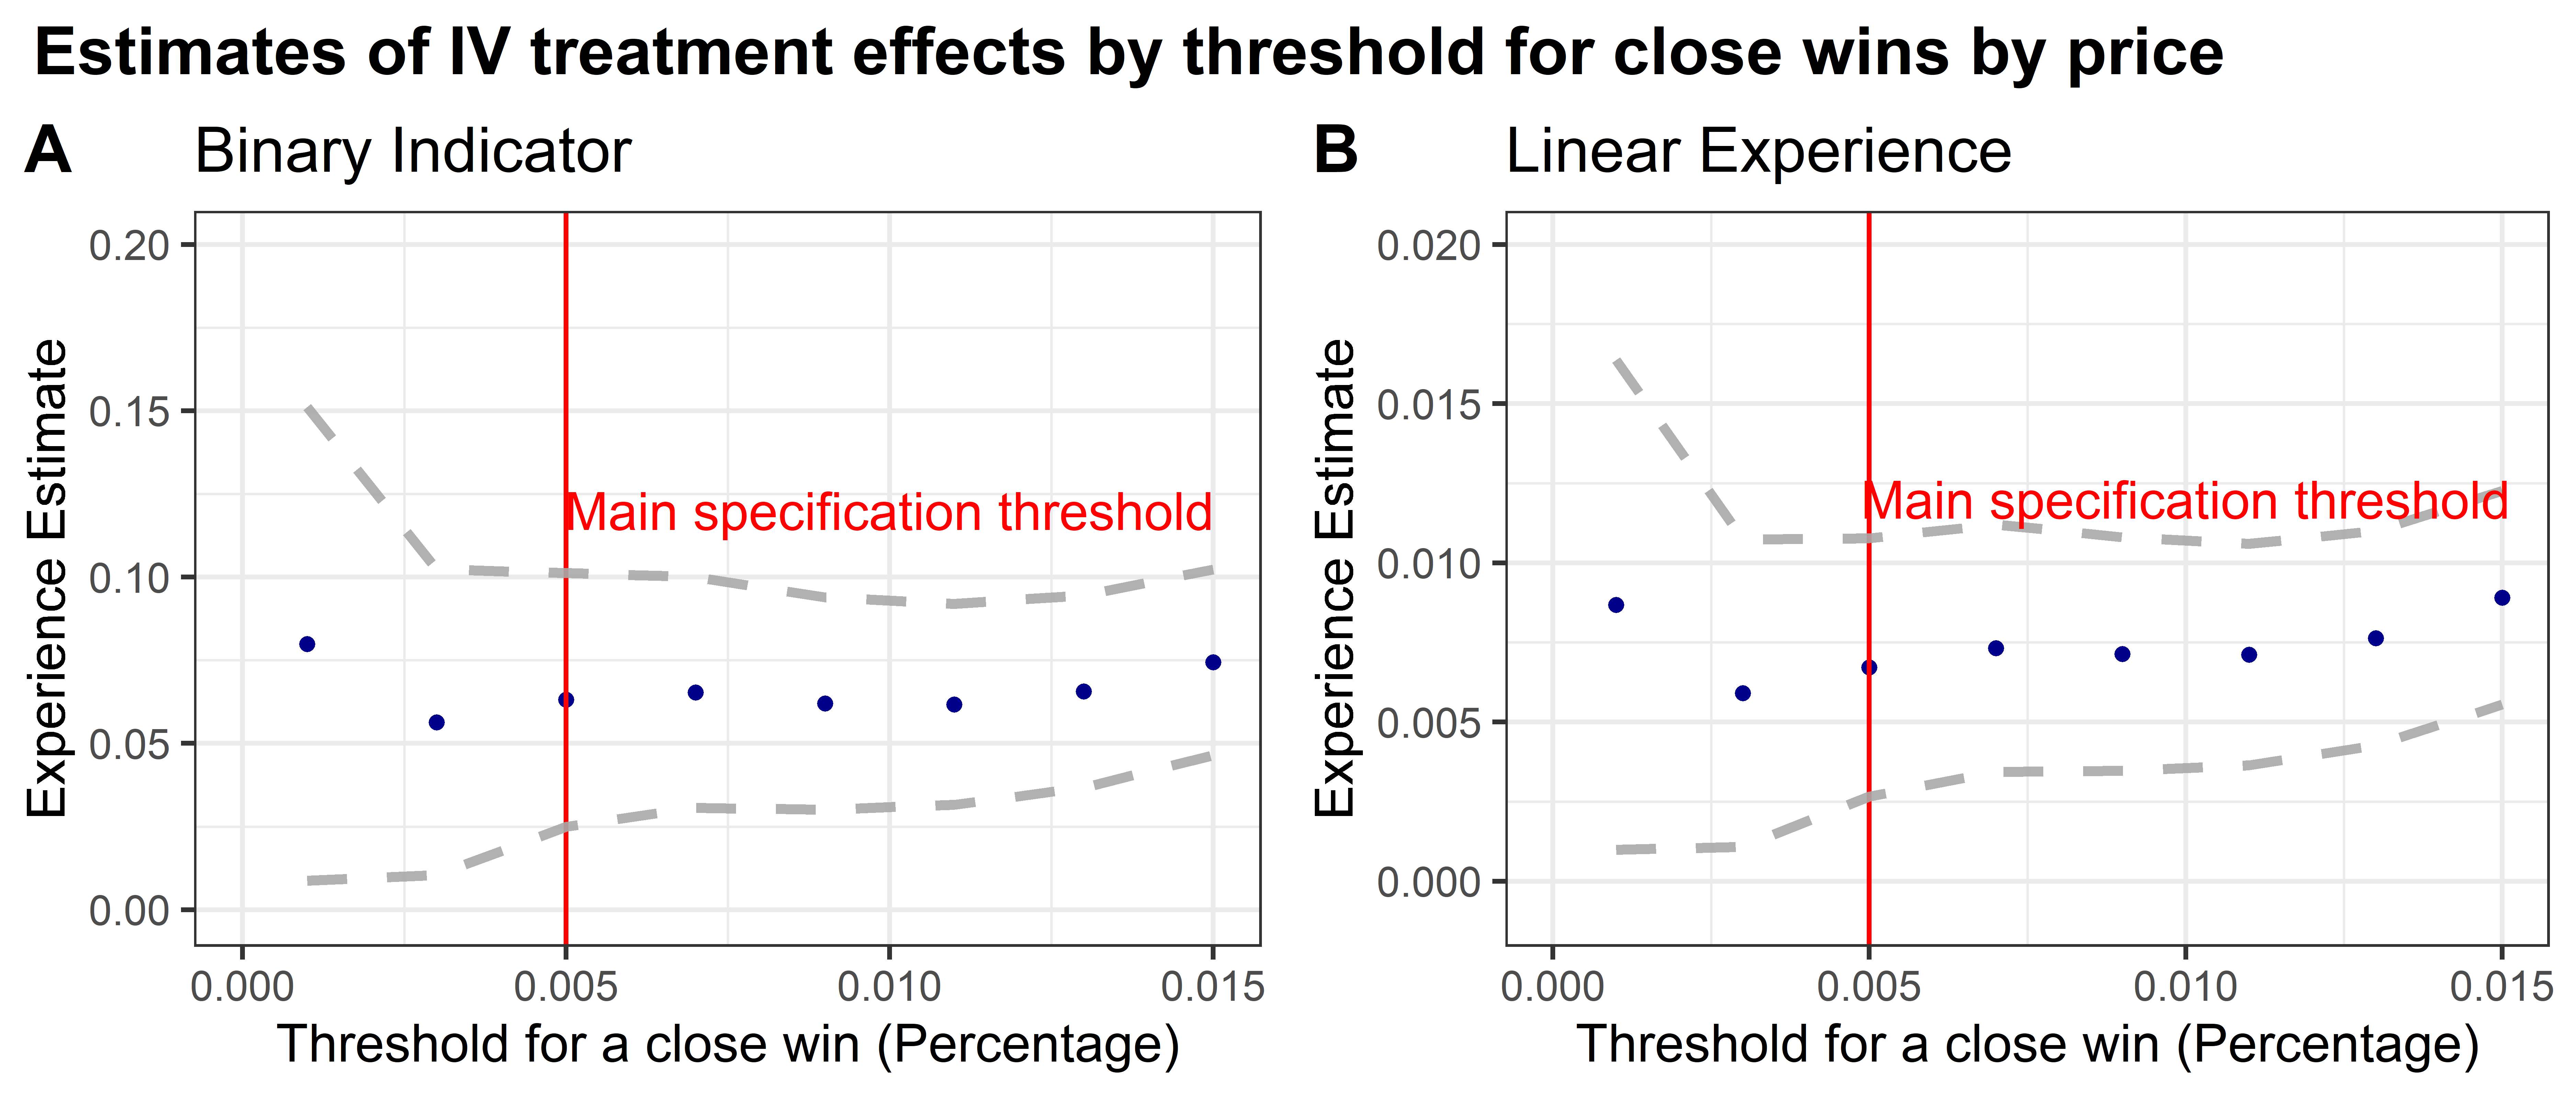
\includegraphics[scale=1]{robustness_threshold.png}
         \caption{Robustness analysis for threshold of close wins}
         \label{fig:close_wins_robust}
     \end{figure}
